%\begin{sidewaysfigure}
%  \begin{center}
%  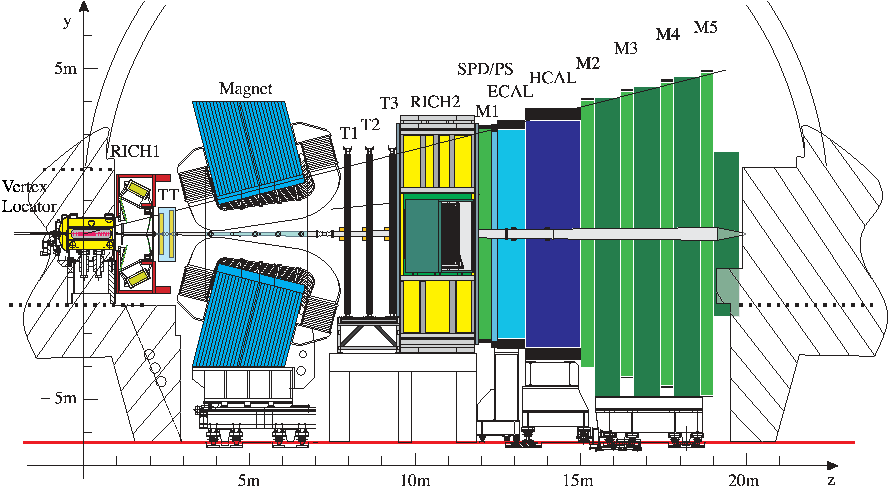
\includegraphics[width=0.8\textheight]{lhcb-detector-cross-section}
%  \caption[Cross-section view of \LHCb, cut in the non-bending $y$--$z$ plane]%
%    {Cross-section view of \LHCb, cut in the non-bending $y$--$z$ plane.}
%  \label{fig:LHCbCrossSection}
%  \end{center}
%\end{sidewaysfigure}



\chapter{The T2K Experiment}
\label{chap:T2KExperiment}
\begin{figure}
  \centering
  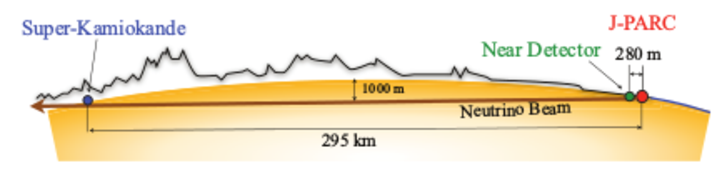
\includegraphics[width=10cm]{images/t2k/t2k_schematic.pdf}
  \caption{The T2K experiment.}
  \label{fig:T2KSchematic}
\end{figure}


The Tokai-to-Kamioka (T2K) experiment~\cite{Abe2011106} is a long baseline neutrino oscillation experiment located in two sites across Japan which was designed to study the parameters governing the PMNS matrix.  The first site is the J-PARC facility in Tokai-mura on Japan's east cost which houses a 30 GeV proton accelerator complex that is used to generate a highly pure $\nu_\mu$ beam.  J-PARC also contains a suite of detectors designed to measure the neutrino beam's unoscillated characteristics.  Super-Kamiokande (SK) is located 295 km (see Fig.~\ref{fig:T2KSchematic}) and measures the contents of the neutrino beam post-oscillation.
\newline
T2K was the first experiment to observe the $\nu_\mu\rightarrow\nu_e$ appearance channel~\cite{PhysRevLett.112.061802} which excluded $\theta_{13} = 0$ at 7.3$\textrm{\sigma}$ significance.  By comparing this result with precise $\theta_{13}$ measurements from reactor experiments, $\textrm{\delta}_{\textrm{CP}}$ regions can be excluded at 90$\%$ confidence level (see Fig.~\ref{fig:NueAppearanceContour}).  T2K's precision analysis of the $\nu_\mu$ disappearance channel provide world leading measurements of $\textrm{\theta}_{23}$ and $\Delta m^2_{23}$.  Independently of the oscillation analyses performed by the experiment, T2K's near detectors, ND280 and INGRID, are used to measure a range of neutrino cross-sections~\cite{PhysRevLett.113.241803, PhysRevD.87.092003}.  While this is not the primary aim of T2K, such measurements are still extremely important as T2K systematic uncertainties can be constrained with additional cross-section knowledge as well as helping to understand the general neutrino interaction picture.

\begin{figure}
  \centering
  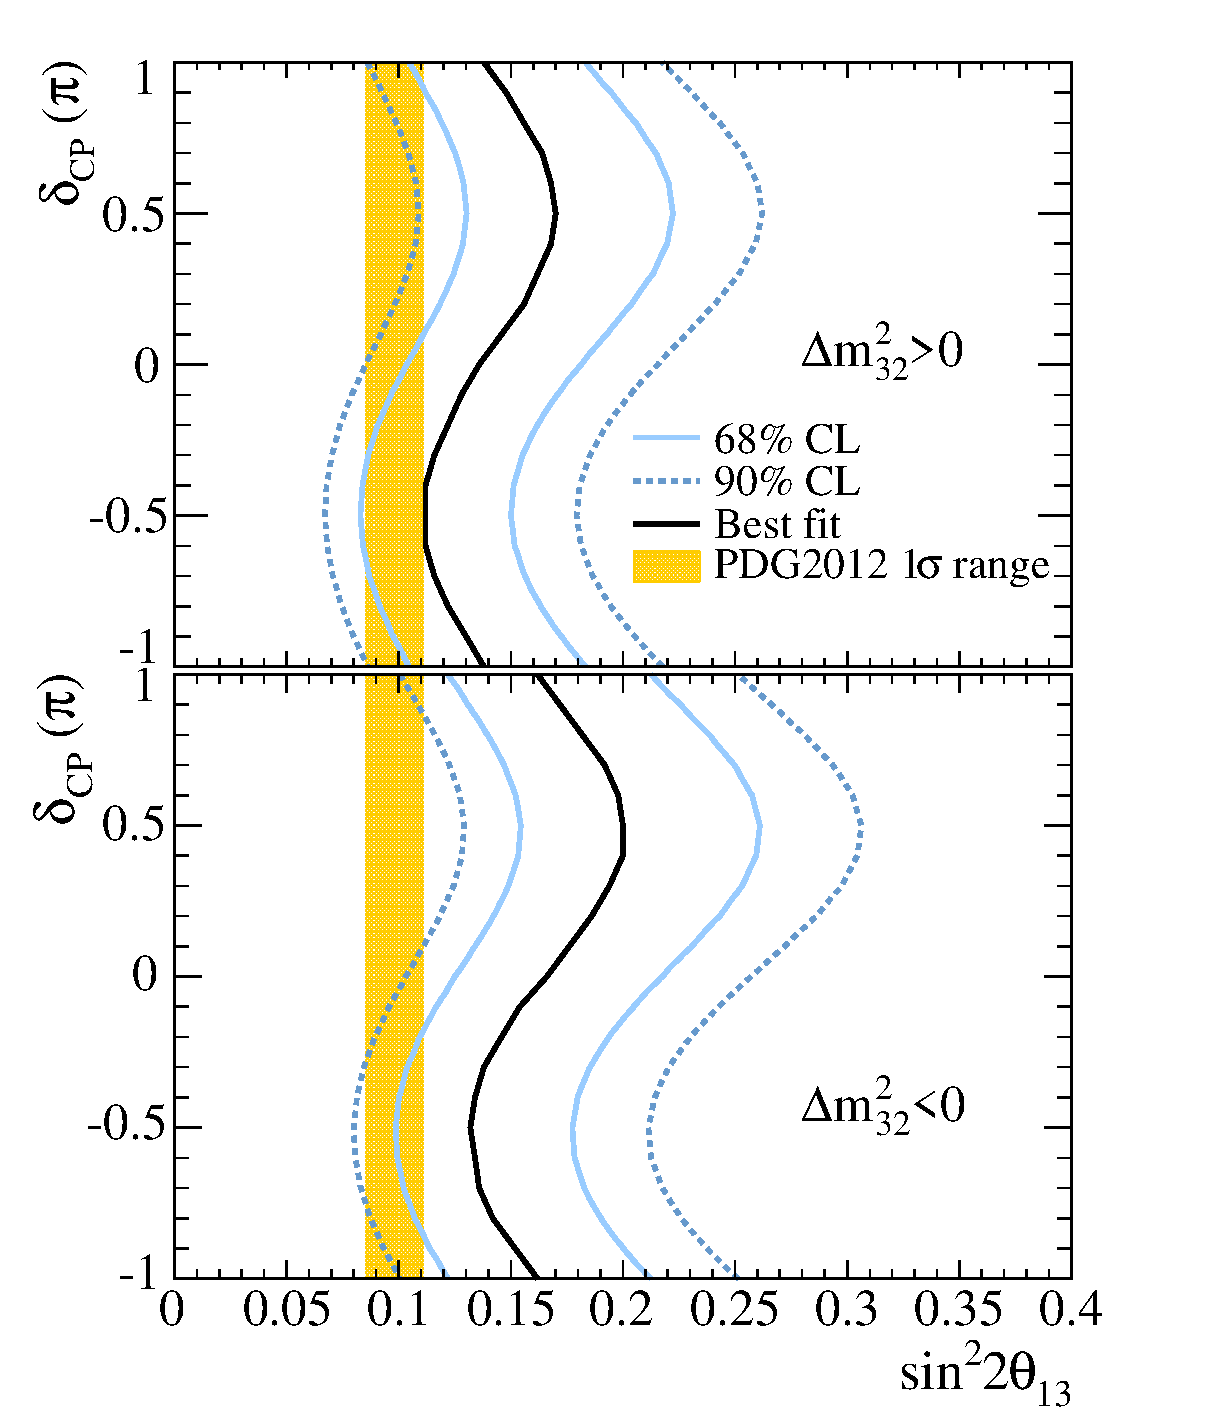
\includegraphics[width=7.5cm]{images/t2k/nue_appearance_Theta13Delta_contour.eps}
  \caption{The 68$\%$ and 90$\%$ confidence level allowed regions for $\sin^22\theta_{13}$ as a function of $\textrm{\delta}_{\textrm{CP}}$ for normal hierachy (top) and inverted hierarchy (bottom)  The solid line represents the best fit $\sin^22\theta_{13}$ for a given $\textrm{\delta}_{\textrm{CP}}$.  The shaded region shows the average $\theta_{13}$ provided by the reactor constraint~\cite{PhysRevLett.112.061802}.}
  \label{fig:NueAppearanceContour}
\end{figure}


\section{T2K beam}
\label{sec:T2KBeam}
The T2K neutrino beam is generated by J-PARC's accelerator complex which produces a 30 GeV proton beam which is fired at a fixed graphite target.  The final-state particles of interactions with the target are predominately charged pions which decay to produce the neutrino beam.  Surrounding and behind the graphite target are a set of magnetic horns which focus the pions into a beam, resulting in a focused neutrino beam after the hadrons have decayed.

\subsection{Accelerator complex}
\label{subsec:AcceleratorComplex}
The J-PARC acclerator complex consists of three sections: the LINnear ACcelerator (LINAC), the Rapid-Cycling Synchotron (RCS) and the Main Ring synchotron (MR).  Production of the proton beam starts at the LINAC where H$^-$ anions are accelerated to 181 MeV which are subsequently converted to h$^+$ ions via charge-stripping foils at the RCS injection point.  With a 25 Hz cycle, the ions are further accelerated by the RCS to 3 GeV with two bunches per cycle.  Roughly 5$\%$ of the proton bunches are fed into the MR where the final acceleration to 30 GeV occurs in bunches of eight.  Extraction of the bunches occurs at two points for different experiments.  For T2K, all eight bunches are extracted in a single turn by five kicker magnets and aimed down the neutrino beamline to the graphite target.  The extraction of all eight bunches forms a single beam spill with a width of 5 $\mu$sec.  The tight structure of the beam spills is vital for background discrimination in the downstream detectors.

\subsection{Neutrino beamline}
\label{subsec:NeutrinoBeamline}

\begin{figure}
  \centering
  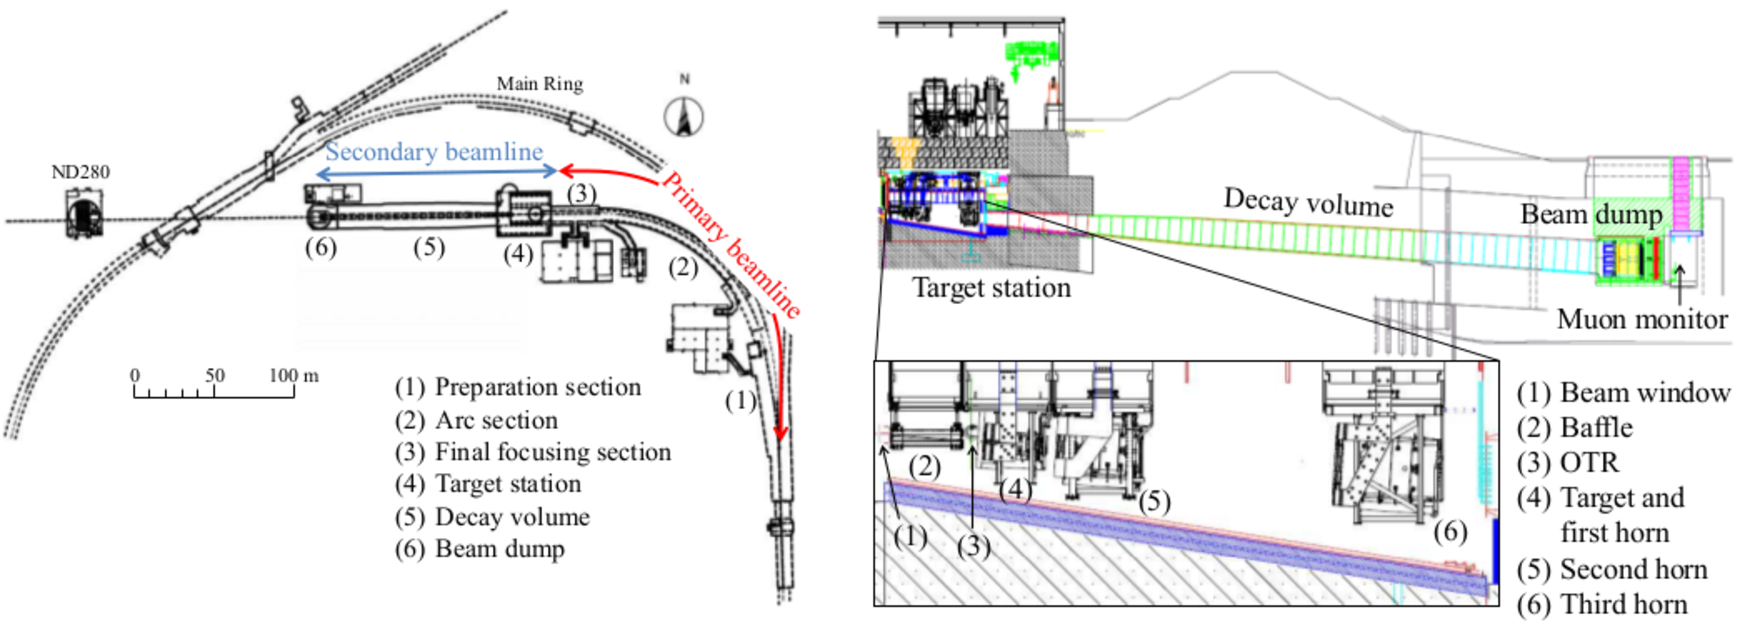
\includegraphics[width=15cm]{images/t2k/neutrino_beamline.pdf}
  \caption{A schematic of the T2K neutrino beamline (left) and a side view of the secondary beamline (right).}
  \label{fig:NeutrinoBeamline}
\end{figure}

The neutrino beamline (NU) is split into a primary and secondary beamline, a schematic of which is shown in Fig.~\ref{fig:NeutrinoBeamline}.  The primary beamline consists of a preparation section, an arc section and a focussing section.  The preparation section uses 11 normal conducting magnets to tune the proton beam for entry into the arc section where the proton beam is bent to its intended direction.  As will be discussed in more detail in section~\ref{subsec:OffAxisBeam}, the axis of the beam is 2.5$^\circ$ away from SK.  The final focussing sections then guides the proton beam into the secondary beamline and the graphite target.
\newline
Sound performance of the proton beam is vital for stability of the T2K neutrino beam.  To ensure such performance, the primary beamline is equipped with a suite of monitors to measure the position, profile, loss and intensity of the proton beam.  The beam position is measured by 21 electrostatic monitors (ESMs) which consists of four cylindrical electrodes surrounding the beam.  The asymmetry of the beam is measured by the induced current in the electrodes is used to infer the position in a non-destructive manner.  Segmented secondary emission monitors (SSEMs) are used to measure the beam loss.  Each SSEM has an anode foil sandwiched between two titanium foil strips.  Protons interact with the strips causing an emission of electrons which electrically drift inducing a current in the strips.  The charge distribution is used to reconstruct the profile.  The beam loss monitors (BLMs) are Ar-CO$_2$ filled wire proportional counters and are used to for beam loss.  The intensity of the beam is measured by five current transformers (CT) which consist of a 50-turn toroidal coil around a ferromagnetic coil.  Passage of the beam induces a current in the coil which is used to infer the number of protons in the spill.  The final CT (CT5) is positioned at the end of the focussing section of the primary beamline and is used to count the number of protons incident on the graphite target.  The accumulated number of protons on target (POT) is used as a metric for the data collected by T2K.  The total POT accumulated so far by T2K is shown in Fig.~\ref{fig:POTHistory}.
\begin{figure}
  \centering
  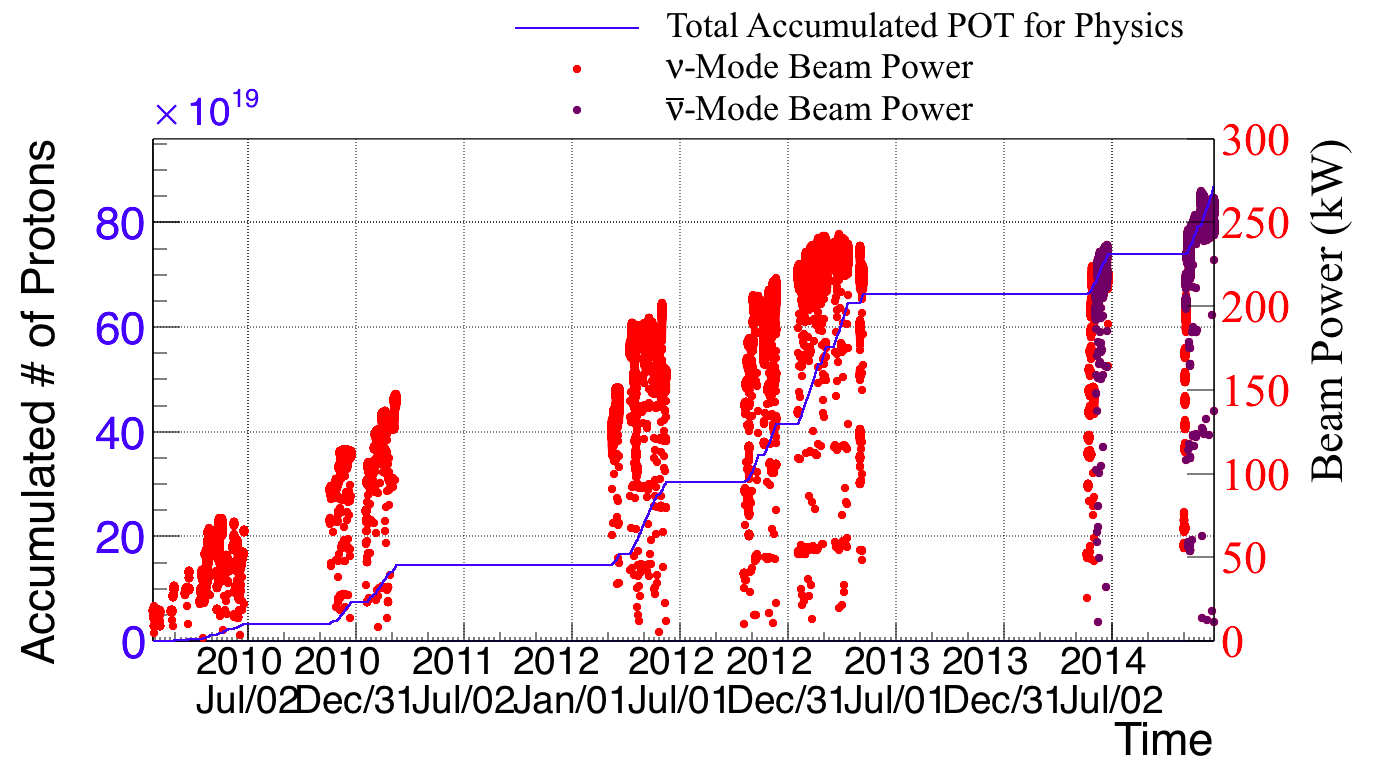
\includegraphics[width=15cm]{images/t2k/pot_history.png}
  \caption{The POT recorded by CT5 as a function of time (blue line) and the recorded beam power in $\nu$ running mode (red dot) and $\bar{\nu}$ running mode (purple dot).}
  \label{fig:POTHistory}
\end{figure}
\newline
The secondary beamline consists of the graphite target, a set of magnetic focusing horns, a decay pipe and a beam dump.  A schematic for the secondary beamline is shown in Fig.~\ref{fig:NeutrinoBeamline}.  The graphite target is a 2.6 cm diameter and 91.4 cm long rod which is surrounded by a 2 mm thick graphite tube and a 0.3 mm titanium case.  The proton-graphite interactions produce charged pions and kaons which are focussed by three magnetic horns, one of which surrounds the target.  The magnetic horns consist of two coaxial conductors which generate a magnetic field with a strength inversely proportional to the distance from the beam axis.  The current direction in the magnetic horns causes the induced field to focus or deflect particles depending on their charge sign.  This simple control allows T2K to operatre in $\nu$ or $\bar{\nu}$ beam mode.  The focused mesons then travel down a decay pipe filled with Helium to reduce pion absorption.  It is here that the mesons decay to produce the neutrinos used as the T2K beam.  To stop measurement contamination, other decay products must be stopped before reaching the downstream detectors.  So, a 75 ton graphite beam dump is positioned at the end of the decay volume.  The beam dump stops almost all non-wanted decay products, with only 5 GeV or above muons successfully propagating through.  As the muons are generally simultaneously produced with the beam neutrinos, measurements of the muon can be used to monitor the direction of the neutrino beam.  To do this, a muon monitor (MUMON) is installed at the downstream end of the beam dump.

\subsection{Off-axis beam}
\label{subsec:OffAxisBeam}
The kinematics of the pion decays dictate the energy spectrum shape of the neutrinos.  Specifically, the peak width of the neutrino energy narrows and shifts as an observer moves off-axis from the pions trajectory.  As the pions are the neutrino parents in the T2K beam, the same effect can be seen by moving off-axis from the neutrino beam.  This effect is illustrated in Fig.BLAH.  By positioning T2K's baseline detectors at 2.5$^\circ$ off-axis, it is possible to align the neutrino beam's peak energy with the first oscillation maximum for the $\nu_\mu$ disappearance channel.  Separately, an off-axis configuration reduces the beam's unwanted high energy tail, improving sensitivity to $\nu_e$ appearance and $\nu_\mu$ disappearance.


\section{Near detector complex}
\label{sec:NearDetectorComplex}
Located 280~m downstream of the beam target is the near detector complex which houses a pair of detectors which measure the unoscillated characteristics of the beam.  The two detectors, named INGRID and ND280, sit in a 37~m deep, open air pit lined with concrete which is surrounded by sand.

\subsection{Multi-Pixel Photon Counter}
\label{subsec:MPPC}
Multi-Pixel Photon Counters (MPPCs)~\cite{1748-0221-4-04-P04004} are used extensively in both INGRID and ND280 for detection of scintillation light during particle energy deposition in plastic scintillator.  The choice of MPPCs, rather than more traditional photomultiplier tubes, was largely due to their ability to operate in a magnetic field.  A MPPC is a multi-pixel avalanche photodiode which consists of 667 pixels over an area of $1.3\times1.3$~mm$^2$.  In terms of operation, each MPPC is held at 0.8-1.5~V above their breakdown voltage, resulting in a gain of $1\times10^6$, which is consistient with the gain of a vacuum photomultiplier~\cite{Abe2011106}.  When light is incident on an MPPC, each pixel acts as a detector for a single photon which means the total signal collected is simply the sum of the MPPC's fired pixels.
\newline
\newline
The scintillator bars, which the MPPCs collect the light from, consist of plastic scintillator bars with a wavelength shifting (WLS) fibre threaded through the centre.  During energy deposition, the plastic scintillator emits photons which are collected and transported by the WLS fibre to the bar's end where the MPPC is located.  The WLS fibre has a twofold purpose: carry the light to the MPPC and shift the spectrum of the light to a region where MPPC detection is optimised.

\subsection{INGRID}
\label{subsec:INGRID}
INGRID (Interactive Neutrino GRID) is one of T2K's near detectors.  With its centre positioned on the beam axis, INGRID is designed to directly monitor the beam's direction and intensity.  INGRID consists of 14 identical modules arranged in a cross formation with two additional modules positioned off-axis towards the end of each horizontal arm (see Fig.~\ref{fig:INGRIDSchematic}).  The cross arrangement allows INGRID to sample the beam in a 10~m $\times$ 10~m transverse section.
\begin{figure}
  \centering
  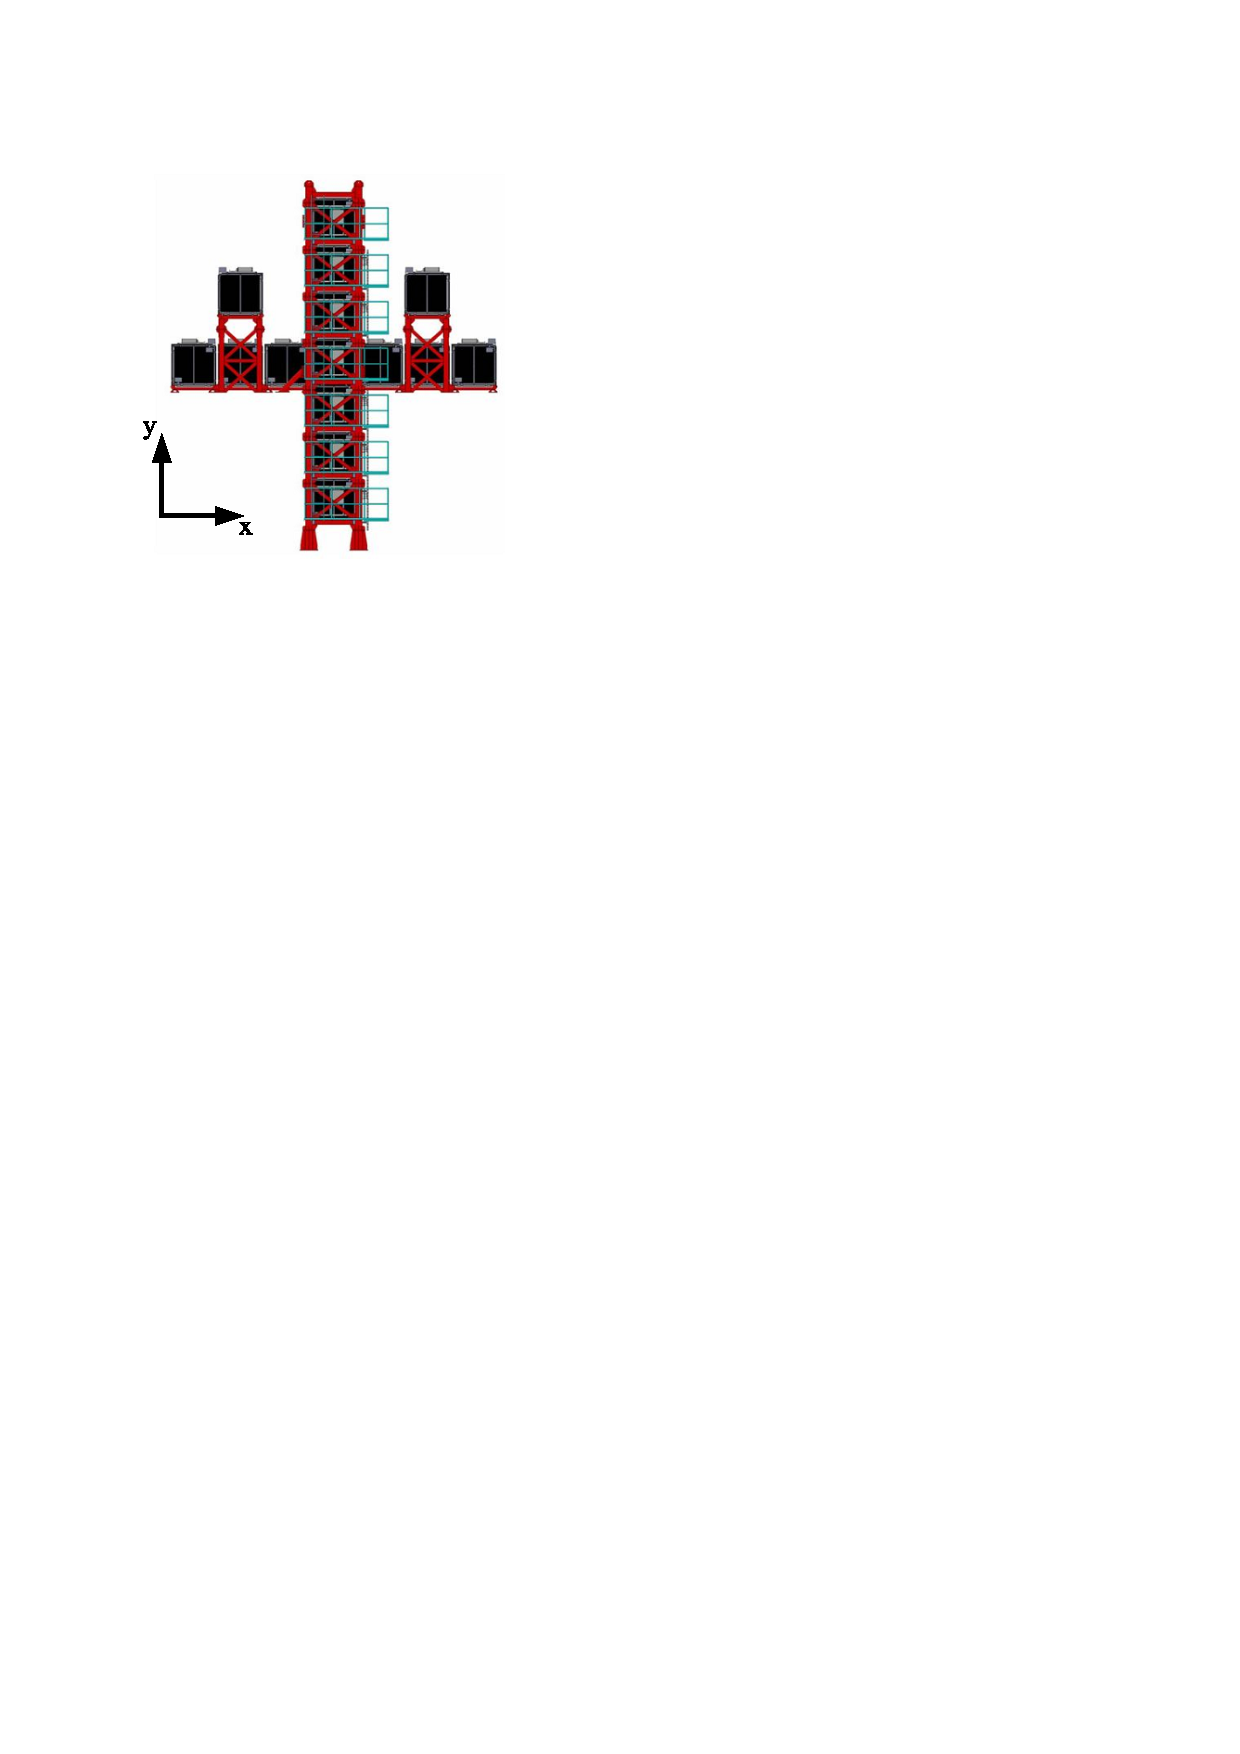
\includegraphics[width=6cm]{images/t2k/INGRID.pdf}
  \caption{A schematic of INGRID.}
  \label{fig:INGRIDSchematic}
\end{figure}
\newline
\newline
Each module consists of nine iron plates and 11 tracking scintillator planes in a sandwich structure.  The iron plates 124~cm $\times$ 124~cm $\times$ 6.5~cm and provide 7.1~tons of target per module for the neutrino beam.  The scintillator planes provide tracking for the neutrino final-states and consist of scintillator bars threaded by WLS fibres and readout by MPPCs (see section~\ref{subsec:MPPC}).
\newline
\newline
This overall design allows INGRID to measure the beam centre to a 10~cm precision which corresponds to 0.4~mrad precision at the near detector complex~\cite{Abe2011106}.


\subsection{ND280}
\label{subsec:ND280}
ND280 (Near Detector at 280~m) is T2K's other near detector.  However, unlike INGRID, ND280 is positioned 2.5$^\circ$ off-axis to the neutrino beam.  ND280 is a heavy, fine-grained detector  which characterises the flux, energy spectrum and $\nu_e$ contamination of the $\nu_\mu$ beam and additionally makes neutrino cross-section measurements.  Because ND280 sits at the same off-axis angle as T2K's far detector, ND280's beam characterisation can be used to make signal and background predictions at the far detector.
\begin{figure}
  \centering
  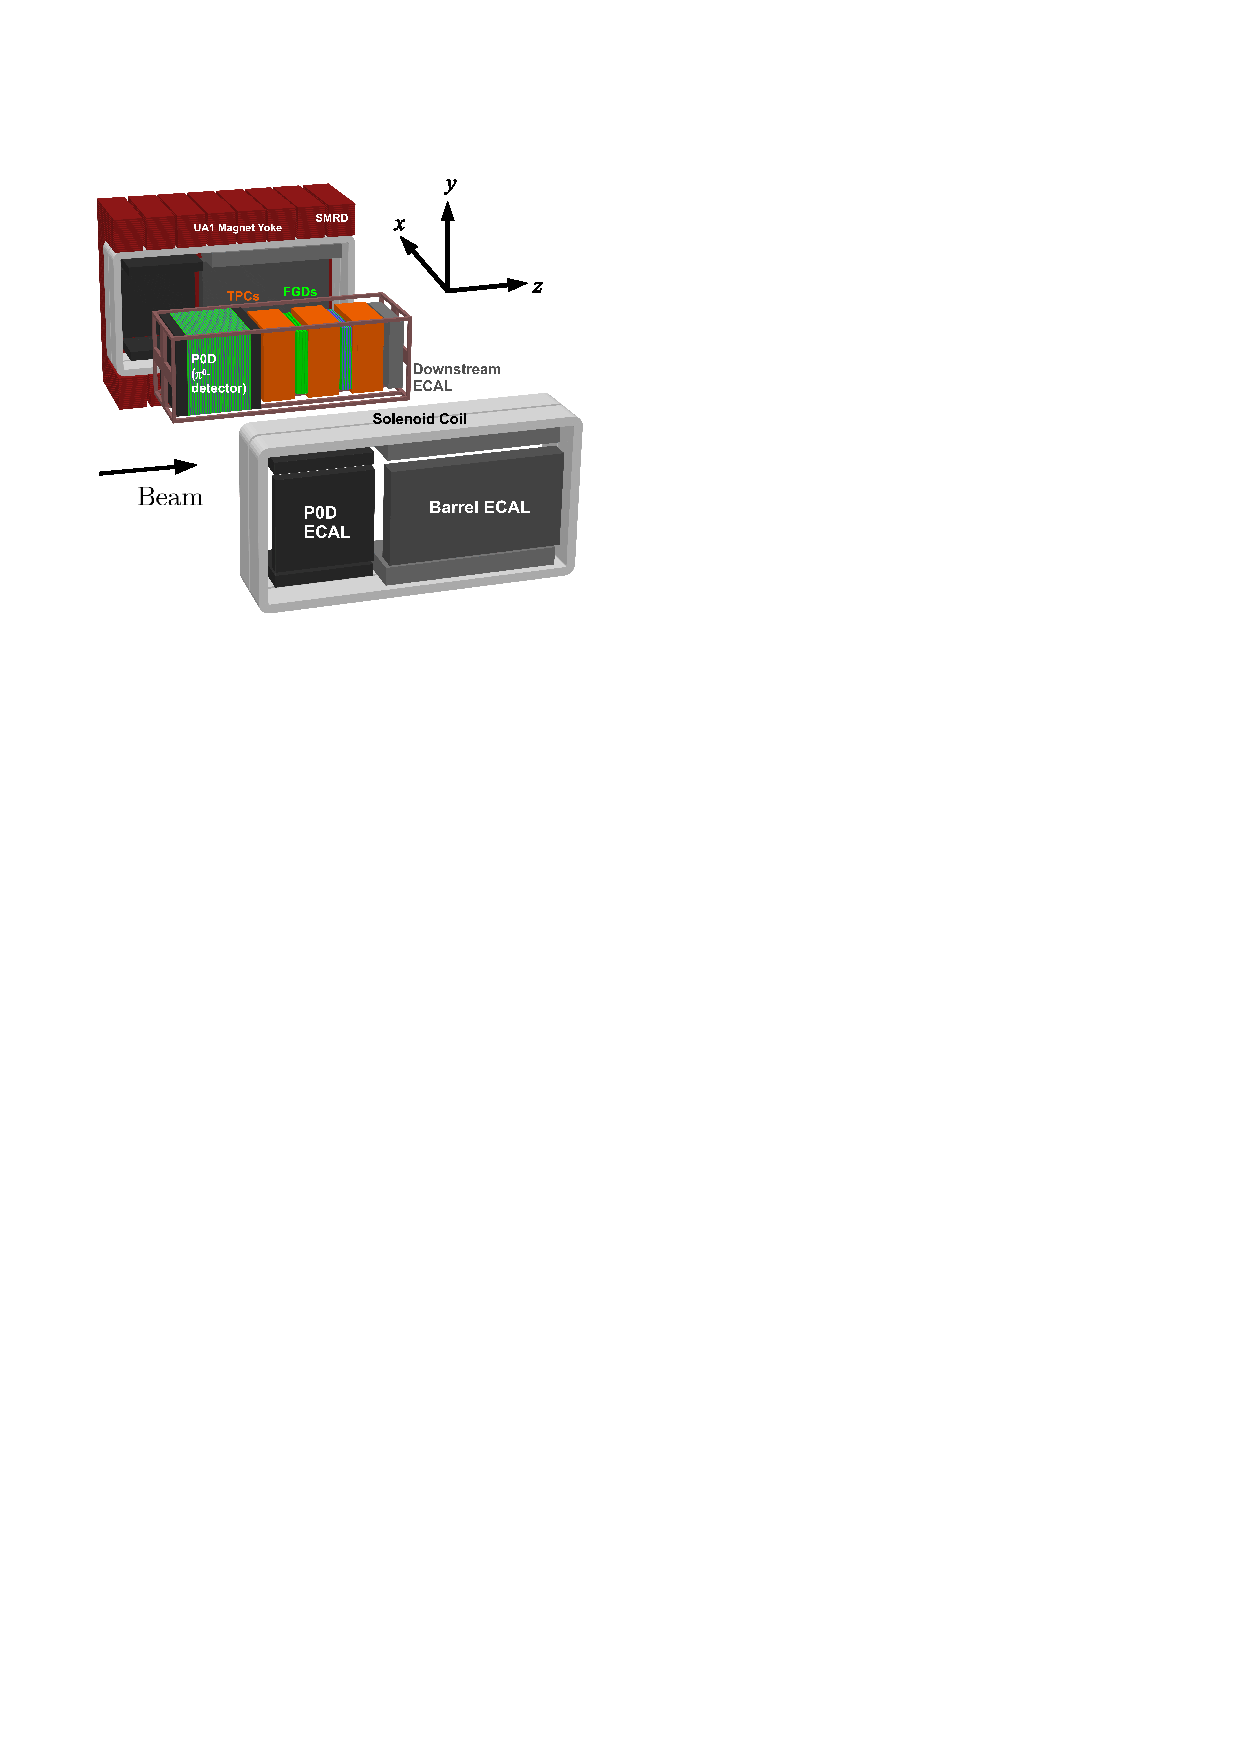
\includegraphics[width=9cm]{images/t2k/ND280Schematic.pdf}
  \caption{An exploded view of ND280~\cite{Abe2011106}.}
  \label{fig:ND280Schematic}
\end{figure}
\newline
\newline
Fig.~\ref{fig:ND280Schematic} shows an exploded view of the detector, which reveals the many subdetectors that form ND280.  The central tracking region comprises two Fine-Grained Detectors (FGDs~\cite{Amaudruz20121}) sandwiched between three Time Projection Chambers (TPCs~\cite{Abgrall201125}). The FGDs, which are composed of layers of plastic scintillator bars, provide the primary target for the neutrinos to interact and the TPCs, filled with a gaseous mixture, allow for tracking of the charged final-states.  Essentially, the detectors in this region are complimentary and their combined information is used to reconstruct the majority of beam events relevant for oscillation analyses.  Upstream of the tracker region lies the $\pi^0$ detector (P$\O$D~\cite{Assylbekov201248}), whose design is optimised studying neutrino interactions with $\pi^0$ in the final-state and consists of layers of scintillator, water and brass.  Surrounding the tracker and P$\O$D are a set of Electromagnetic Calorimeters (ECals~\cite{1748-0221-8-10-P10019}), primarily designed to detect particles originating from ND280's inner region.  Because particle identification is paramount to ND280's physics goals, all of the above detectors sit in a constant 0.2~T magnetic field, which is aligned with the $x$-axis in Fig.~\ref{fig:ND280Schematic}.  The magnetic return yoke and coils used to generate this field emcompass the entire detector, allowing a constant field to be maintained within the detector, but greatly minimising the field's outside extent.  To maximise ND280's physics capability, the magnetic return yoke is instrumanted with layers of plastic scintillator, which form the Side Muon Range Detectors (SMRDs~\cite{Aoki2013135}).


\subsubsection{The electromagnetic calorimeters}
\label{subsubsec:ecal}
The ND280 ECal is a lead-scintillator sampling calorimeter which conists of 13 modules separated into three distinct regions: the P$\O$D ECal which consists of six modules surrounding the P$\O$D, the barrel-ECal which is separated into six modules surrounding the tracker region and the DownStream-ECal (DS-ECal) which is a single module located downstream of the inner detectors.  Motivated by their physics goals, the barrel-ECal and DS-ECal are often considered together and will be referred to as the tracker ECal, while the P$\O$D ECal is considered a separate detector which is not used in this analysis and so will not be discussed further.  The primary physics goal of the ECal is to aide particle identification for final-states originating in the central region of ND280.  This is particularly important for interactions with $\pi^0$ in the final-state as the decay photons are difficult to identify using the tracker alone.
\newline
\newline
%All modules in the tracker ECal consist of layers of scintillating polystyrene bars with a 40~mm $\times$ 10~mm cross-section bonded to 1.75~mm lead sheets.
The barrel-ECals are separated into six modules: two modules above the tracker, two either side of the tracker and two below the tracker.  Each barrel-ECal module consists of layers of scintillating polystyrene bars with a 40~mm $\times$ 10~mm cross-section bonded to 1.75~mm lead sheets.  The scintillator bar provide a means of tracking the final-states while lead sheets act as a radiator to produce electromagnetic showers and additionally provide a heavy mass neutrino target.  To measure the light readout, each scintillator bar has a 2~mm hole running through the centre in which a WLS fibre is inserted.  The fibre carries the light to the end of the bar where it can be collected by an MPPC.  The size of the gap between the tracker and the magnet placed a strong constraint on the size of barrel modules and so a scintillator bar thickness of 10~mm was chosen to minimise the ECal depth while maintaining a bar thickness which could provide sufficient light for signal capture.  The other key features of the active barrel-ECal volume, bar thickness, lead thickness and number of layers) was chosen to optimise particle identification and tracking.  A smaller bar width results in a detector with a higher resolution and studies investigating this found that the $\pi^0$ reconstruction efficiency was greatly compromised for $>$50~mm bar widths.  So, to facilitate costings, a compromise bar width of 40~mm was chosen.  The thickness of the lead absorber says was also optimised based on the $\pi^0$ reconstruction efficiency.  The number of scintillator-lead layers was chosen such that electromagnetic showers of energy up to 3~GeV were adequately contained.  It was found that 10 electron radiation lengths ($X_0$) were required to ensure at least 50$\%$ of $\pi_0$ decay photon showers were contained.  So, this motivated a choice of 31 layers for all barrel-ECal modules which is equivalent to 9.7$X_0$.  For the purpose of 3D reconstruction, each ECal layer is oriented at 90$^\circ$ to the previous layer.  This means that in all barrel modules, there are 16 layers perpendicular and 15 layers parallel to the beam direction.  The perpendicular and parallel layers are slightly different, in that the scintillator bars are a different length.  In all barrel modules, the parallel bars are 3840~mm and are read out at both ends by separate MPPCs.  Because of the geometry, this is not the case for the perpendicular bars; the top and bottom module bar lengths are 1520~mm whereas the side module bar lengths are 2280~mm.  For all perpendicular bars, the signal is read out at one end only with the other end mirrored with aluminimum to reflect the light.  Each barrel module is sandwiched between two carbon fibre plates and held in an aluminium frame which provides secure, structural support.
\newline
\newline
The DS-ECal has almost identical features to that of the barrel in that it has scintillator bars with an identical chemical composition and cross-section while the lead absorbers are equally thick.  However, unlike the barrel-ECals, the DS-ECal consists of 34 lead-scintillator layers which are, again, orientated at 90$^\circ$ to the previous layer.  Because of this, the DS-ECal has a radiation length of 10.6$X_0$.  Additionally, every scintillator bar is 2000~mm and is read out at both ends by MPPCs.  Also, because of its position in the geometry, all layers are perpendicular to the beam direction.  The carbon fibre plates and aluminium frame are identical to those used in the barrel-ECal.
\newline
\newline
A summary of the tracker-ECal design is shown in table.~\ref{table:ECalDesign}.
\begin{table}
\begin{center}
\begin{tabular}{l|l|l}
\hline
        & DS-ECal  &Barrel ECal  \\ \hline
Length (mm)& 2300      & 4140   \\ 
Width (mm)  & 2300      & 1676  top/bottom \\ 
        &          & 2500 side  \\ 
Depth (mm)  & 500     & 462    \\
Weight (kg) & 6500 & 8000 top/bottom  \\
            &      & 10000 side        \\ \hline
Num. of layers &  34      &  31  \\ \hline
Bar orientation & $x/y$ &Para. and Perp \\ \hline
Num. of bars    & 1700     & 2280 Para. top/bottom  \\ 
        &          & 1710 Para. sides \\     
        &          & 6144 Perp top/bottom   \\ 
        &          & 3072 Perp sides       \\ \hline  
Bars per layer & 50 & 38 Para. top/bottom\\
               &    & 57 Para. side\\
               &    & 96 Perp top/bottom/sides  \\  \hline
Bar length (mm) & 2000  & 3840  Para. \\ 
           &      & 1520 Perp top/bottom \\ 
           &      & 2280 Perp sides      \\ \hline
Pb thickness (mm) & 1.75  & 1.75    \\ \hline 
\end{tabular}
\caption{Summary of the ECal design showing the overall dimensions, numbers of layers, length and orientation ofscintillator bars, numbers of bars, and lead thickness for each module~\cite{1748-0221-8-10-P10019}.}
\label{table:ECalDesign} 
\end{center}
\end{table}
\newline
\newline
The scintillator bars consist of polystyrene doped with 1$\%$~PPO and 0.03$\%$~POPOP and were extruded at a dedicated Fermilab facility.  During charge deposition, the PPO works as the primary scintillator and its output photons result in secondary scintillation of the POPOP.  This process acts as a wavelength shifter to produce an emission peak of 420~nm which matches the absorption peak of the 1~mm dimaeter WLS fibre threaded through the centre of the bar.  Every tracker-ECal bar contains a 0.25~mm coating of polystyrene co-extruded with TiO$_2$ which provides reflection of the scintillation light.
\newline
\newline
The lead aborber layers consist of naturally occurring lead and stiffened with 2$\%$ antimony.  Traces of other metals are present but are below 0.15$\%$.  During construction, each lead layer was coated with a black, quick drying metal-conditioning primer to protect personnel from the toxic effects of the lead and to prevent leaching into the scintillator bars.  The lead layers themselves are actually constructed from multiple sheets rather than a single sheet largely due to ease of transportation.  In the case of the DS-ECal, each layer consists of two 1008~mm $\times$ 2016~mm sheets.  For the top and bottom ECal modules, each layer consists of two 765~mm $\times$ 3858~mm sheets and the side module aborbers are constructed from four 2330~mm $\times$ 964.5~mm sheets.
\newline
\newline
The tracker-ECal electronics system consists of several different readout boards.  All MPPCs are connected to a set of bespoke Trip-T Frontend Boards (TFBs).  Each TFB comes with 64 channels to read out MPPCs which means that there are multiple TFBs associated with each ECal module.  All TFBs subsequently connected to Readout Merger Modules (RMMs) which act as the interface between the Data AQuisition system (DAQ) and its associated TFBs.

\subsubsection{Data aquisition system}
\label{subsubsec:DAQ}
ND280 comes equipped with a DAQ which is responsible for triggering the readout of information from the subdetectors and subsequent storage.  Because of the low frequency of neutrino events, there are no strict trigger requirements which is in start contrast to collider experiments.  So, there are only three triggers which are:
\begin{itemize}
\item \textbf{Beam trigger:} When a beam spill occurs, a signal is timing signal is set to the DAQ which issues a command to record ND280 data. 
\item \textbf{TRIP-t cosmic trigger:} If hits are seen on opposite sides of the outer detector (allowed combinations are top and bottom SMRD, left and right SMRD, P$\O$D and DS-ECal) which are outside of the beam time window, then the DAQ records data as the hits were likely caused by a cosmic ray muon.
\item \textbf{FGD cosmic trigger:} If hits are seen in both FGDs which are outisde of the beam time window, then data is recorded as this was also likely to be caused by a cosmic ray muon.
\end{itemize}
The data is initially stored at KEK in Japan but is then replicated to TRIUMF in Canada and RAL in the UK for maximum redundancy and ease of access.

\subsection{The far detector}
I mean SK



